\section{Methodology}

In this section, we describe the core components of our proposed approach: Delta Packing and its extension to Delta-Based Tile Scoring (DTS). 

\subsection{Delta Packing}
The foundational operation in our methodology is Delta Packing. Adjacent query and key vectors are highly similar at the token level, which means they can be compressed along the sequence dimension. 

Algorithm 1 outlines the sequential Delta Packing procedure.

\begin{figure}[htbp]
\noindent\hrulefill\\
\textbf{Algorithm 1: Sequential Delta Packing}\\[-2mm]
\noindent\hrulefill
\begin{tabbing}
\textbf{Input:} Matrix $\mathbf{K} \in \mathbb{R}^{N \times D}$, similarity threshold $\tau$ \\
\textbf{Output:} Packed matrix $\hat{\mathbf{K}}$, binary mask $\Delta \in \{0, 1\}^N$ \\
1. \quad \= $\Delta \gets \mathbf{0}$, $\Delta[0] \gets 1$ \\
2. \> $\mathbf{k}_{\text{anchor}} \gets \mathbf{K}[0]$ \\
3. \> \textbf{for} $i = 1$ \textbf{to} $N-1$ \textbf{do} \\
4. \> \quad \= \textbf{if} $\cos(\mathbf{K}[i], \mathbf{k}_{\text{anchor}}) < \tau$ \textbf{then} \\
5. \> \> \quad \= $\Delta[i] \gets 1$ \\
6. \> \> \> $\mathbf{k}_{\text{anchor}} \gets \mathbf{K}[i]$ \\
7. \> \> \textbf{end if} \\
8. \> \textbf{end for} \\
9. \> $\hat{\mathbf{K}} \gets \mathbf{K}[\Delta == 1]$ \\
10.\> \textbf{return} $\hat{\mathbf{K}}, \Delta$
\end{tabbing}
\vspace{-4mm}
\noindent\hrulefill
\end{figure}

\textbf{Parallel Delta Packing.}
In practice, we apply sequential delta packing to fixed-size chunks (e.g., 128 tokens) independently by setting each chunk's first vector as an anchor, which breaks the sequential dependency. Otherwise, sequential packing has a linear time complexity with respect to sequence length, which would result in severe overhead in extremely long contexts.



\subsection{Delta-Based Tile Scoring (DTS)}
Building upon the Delta Packing concept, we introduce Delta-Based Tile Scoring (DTS) for block-sparse attention. 

The DTS methodology operates as follows:
\begin{enumerate}
    \item \textbf{Delta Pack:} Apply Delta packing on \textbf{Q} and \textbf{K} separately.
    \item \textbf{Multiply:} Multiply the packed $\hat{\textbf{Q}}$ and $\hat{\textbf{K}}$ to get representative attention scores in tiles.
    \item \textbf{Sum:} Sum the tile attention scores to get an importance score for each tile.
    \item \textbf{Normalize:} Apply softmax to the tile scores across query rows to obtain tile weights.
    \item \textbf{Threshold:} Select the highest-scoring tiles per row until their accumulated weights exceed a threshold $\tau = 0.9$.
    \item \textbf{Compute:} Process the selected tiles using block-sparse attention and skip the remaining tiles.
\end{enumerate}



Figure~\ref{fig:delta_tile_scoring} provides a detailed algorithmic view of how \textbf{Q} and \textbf{K} are packed into $\hat{\textbf{Q}}$ and $\hat{\textbf{K}}$, and how these packed matrices are multiplied to obtain the sparse attention scores.

Figure~\ref{fig:dts_flow} illustrates the complete end-to-end flow of this four-stage methodology, showcasing how the sparse attention scores are summed to compute tile importance, and how these tile scores determine which tiles are processed and which are skipped.

\begin{figure}[!ht]
\centering
\resizebox{\columnwidth}{!}{
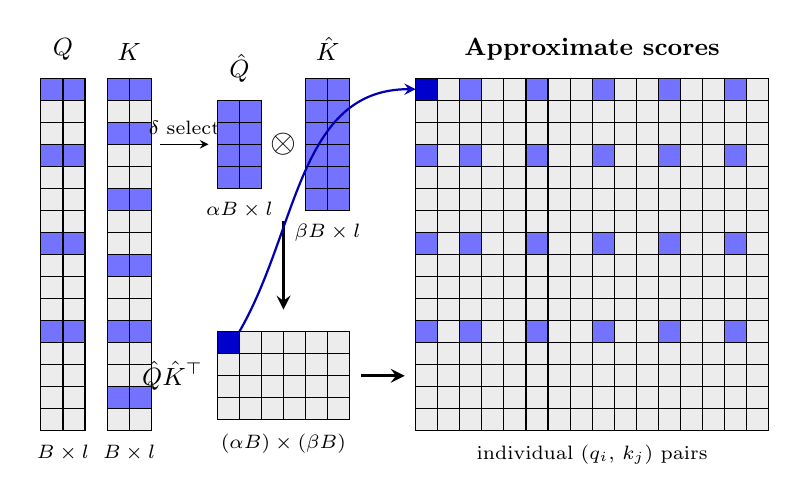
\begin{tikzpicture}
  \def\cell{0.28}
  \colorlet{hilightA}{blue!55}
  \colorlet{hilightFocus}{blue!80!black}
  \colorlet{plain}{gray!15}

  % Q anchors: rows 0, 3, 7, 11   (4 of 16)
  % K anchors: rows 0, 2, 5, 8, 11, 14  (6 of 16)

  %--- Full Q (16 rows × 2 cols) ---
  \foreach \r in {0,...,15} {
    \pgfmathtruncatemacro{\isanchor}{
      (((\r==0)+(\r==3)+(\r==7)+(\r==11))>0) ? 1 : 0
    }
    \foreach \c in {0,1} {
      \ifnum\isanchor=1 \fill[hilightA] \else \fill[plain] \fi
        ({\c*\cell},{-\r*\cell}) rectangle ({(\c+1)*\cell},{(-\r-1)*\cell});
      \draw ({\c*\cell},{-\r*\cell}) rectangle ({(\c+1)*\cell},{(-\r-1)*\cell});
    }
  }
  \node[above, font=\small\bfseries] at ({1*\cell}, 0.1)             {$Q$};
  \node[below, font=\scriptsize]     at ({1*\cell},{-16*\cell-0.05}) {$B \times l$};

  %--- Full K (16 rows × 2 cols) ---
  \foreach \r in {0,...,15} {
    \pgfmathtruncatemacro{\isanchor}{
      (((\r==0)+(\r==2)+(\r==5)+(\r==8)+(\r==11)+(\r==14))>0) ? 1 : 0
    }
    \foreach \c in {0,1} {
      \ifnum\isanchor=1 \fill[hilightA] \else \fill[plain] \fi
        ({(3+\c)*\cell},{-\r*\cell}) rectangle ({(4+\c)*\cell},{(-\r-1)*\cell});
      \draw ({(3+\c)*\cell},{-\r*\cell}) rectangle ({(4+\c)*\cell},{(-\r-1)*\cell});
    }
  }
  \node[above, font=\small\bfseries] at ({4*\cell}, 0.1)             {$K$};
  \node[below, font=\scriptsize]     at ({4*\cell},{-16*\cell-0.05}) {$B \times l$};

  %--- Delta-select arrow ---
  \draw[-{stealth}] ({5.4*\cell},{-3*\cell}) -- ({7.6*\cell},{-3*\cell});
  \node[above, font=\scriptsize] at ({6.5*\cell},{-3*\cell}) {$\delta$ select};

  %--- \hat{Q} (4 rows × 2 cols) ---
  \foreach \r in {0,...,3} {
    \foreach \c in {0,1} {
      \fill[hilightA]
        ({(8+\c)*\cell},{-(1+\r)*\cell}) rectangle ({(9+\c)*\cell},{-(2+\r)*\cell});
      \draw ({(8+\c)*\cell},{-(1+\r)*\cell}) rectangle ({(9+\c)*\cell},{-(2+\r)*\cell});
    }
  }
  \node[above, font=\small\bfseries] at ({9*\cell},{-1*\cell+0.1})       {$\hat{Q}$};
  \node[below, font=\scriptsize]     at ({9*\cell},{-5*\cell-0.05}) {$\alpha B \times l$};

  %--- ⊗ ---
  \node[font=\large] at ({11*\cell},{-3*\cell}) {$\otimes$};

  %--- \hat{K} (6 rows × 2 cols) ---
  \foreach \r in {0,...,5} {
    \foreach \c in {0,1} {
      \fill[hilightA]
        ({(12+\c)*\cell},{-\r*\cell}) rectangle ({(13+\c)*\cell},{-(1+\r)*\cell});
      \draw ({(12+\c)*\cell},{-\r*\cell}) rectangle ({(13+\c)*\cell},{-(1+\r)*\cell});
    }
  }
  \node[above, font=\small\bfseries] at ({13*\cell}, 0.1)       {$\hat{K}$};
  \node[below, font=\scriptsize]     at ({13*\cell},{-6*\cell-0.05}) {$\beta B \times l$};

  %--- Downward Flow Arrow ---
  \draw[-{stealth}, very thick] ({11*\cell},{-6.5*\cell}) -- ({11*\cell},{-10.5*\cell});

  %--- (αB)×(βB) result matrix: 4 rows × 6 cols ---
  \foreach \r in {0,...,3} {
    \foreach \c in {0,...,5} {
      \pgfmathtruncatemacro{\isFocus}{(\r==0)*(\c==0)}
      \ifnum\isFocus=1
        \fill[hilightFocus]
      \else
        \fill[plain]
      \fi
        ({(8+\c)*\cell},{-(11.5+\r)*\cell}) rectangle ({(9+\c)*\cell},{-(12.5+\r)*\cell});
      \draw ({(8+\c)*\cell},{-(11.5+\r)*\cell}) rectangle ({(9+\c)*\cell},{-(12.5+\r)*\cell});
    }
  }
  \node[left, font=\small\bfseries]  at ({7.8*\cell},{-13.5*\cell})    {$\hat{Q}\hat{K}^\top$};
  \node[below, font=\scriptsize]     at ({11*\cell},{-15.5*\cell-0.05}) {$(\alpha B)\times(\beta B)$};

  %--- Rightward Flow Arrow ---
  \draw[-{stealth}, very thick] ({14.5*\cell},{-13.5*\cell}) -- ({16.5*\cell},{-13.5*\cell});

  %--- 16×16 full score matrix ---
  \foreach \r in {0,...,15} {
    \foreach \c in {0,...,15} {
      \pgfmathtruncatemacro{\isHL}{
        (((\r==0)+(\r==3)+(\r==7)+(\r==11))>0) *
        (((\c==0)+(\c==2)+(\c==5)+(\c==8)+(\c==11)+(\c==14))>0)
      }
      \pgfmathtruncatemacro{\isFocus}{(\r==0)*(\c==0)}
      \ifnum\isFocus=1
        \fill[hilightFocus]
      \else
        \ifnum\isHL=1
          \fill[hilightA]
        \else
          \fill[plain]
        \fi
      \fi
        ({(17+\c)*\cell},{-\r*\cell}) rectangle ({(18+\c)*\cell},{-(1+\r)*\cell});
      \draw ({(17+\c)*\cell},{-\r*\cell}) rectangle ({(18+\c)*\cell},{-(1+\r)*\cell});
    }
  }
  \node[above, font=\small\bfseries] at ({25*\cell}, 0.1) {Approximate scores};
  \node[below, font=\scriptsize]     at ({25*\cell}, {-16*\cell-0.05}) {individual $(q_i,\,k_j)$ pairs};

  %--- Arrow from result cell (0,0) to B×B position (0,0) ---
  \draw[-{stealth}, thick, blue!70!black]
      ({9*\cell},{-11.5*\cell})
      to[out=60, in=180]
      ({17*\cell},{-0.5*\cell});

\end{tikzpicture}
}
\caption{Delta-based tile scoring. Delta pre-processing selects content-adaptive anchors (blue) from $Q$ and $K$ independently, producing $\hat{Q}$ and $\hat{K}$. Their product gives an $(\alpha B)\times(\beta B)$ score matrix; each entry (highlighted cell, arrow) corresponds to a single dot product at one position in the full $B\times B$ score tile.}
\label{fig:delta_tile_scoring}
\end{figure}


\subsection{Per-Head $\tau$ Calibration}
A global threshold of $\tau=0.9$ does not strictly guarantee retaining $90\%$ of the true attention mass, because the tile scores are only estimates. To accurately achieve the target retention rate, similar to X-Attention, we perform an offline calibration step. During this step, the threshold $\tau$ is independently tuned for each attention head so that every head reliably retains its target mass. Detailed procedures for this calibration are presented in Appendix~\ref{app:calibration}.
